\section{Auswertung der Messungen bei 25$^\circ$C}

Mit den erhalten Messwerten aus Teil 1 kann jetzt die Konzentrationsabhängigkeit der Essigsäure im Hinblick auf:

\begin{itemize}
    \item den mittleren Aktivitätskoeffizient $\gamma_\pm$
    \item den Dissoziationsgrad $\alpha$
    \item und den Debye-Radius (\textbf{rD})
\end{itemize}

untersucht werden.

\subsection{Bestimmung der Aktivitätskoeffizienten $\gamma_\pm$ bei 25$^\circ$C}

Um dem Phänomen des schwachen Elektrolyten rechnung zu tragen, bei dem nur ein geringer Teil der Essigsäuremoleküle dissoziiert und ein $H^+$ abgibt,
wurde die Aktivität $a$ eingeführt. Dieser Wert sagt aus, wie viele Moleküle wirklich regieren. 
Da wir über die pH-Messung den negativen dekadischen Logarithmus der $H^+$-Ionenkonzentration in Lösung bestimmt haben, erhalten wir durch potenzieren
zur Basis 10 genau die Zahl an Teilchen, die in unserer Lösung dissoziiert ist.

\begin{align}
    a = 10^{pH-Wert}
\end{align} 

Da mit $a$ immer nur der absoluten Zahlenwert für eine ganz bestimmte Lösung bestimmt werden kann, wurde der mittlere Aktivitätskoeffizient $\gamma_\pm$
eingeführt, da dieser jetzt das Verhältnis zwischen der reagierten Spezies und der eingesetzten Konzentration berechnet, bekommt man immer das
gleiche Ergebnis auch wenn man das System vergrößert oder verkleinert.

\begin{align}
    \gamma_\pm = \frac{a}{c} = \frac{a}{b}
\end{align}

Da unsere Konzentrationen in Molalität statt in Molarität gegeben sind wird Anstell $c$ $b$ für die Konzentration eingesetzt. \\
Für den prozentualen Anteil an dissoziierten Teilchen wird noch $\alpha$ mit:

\begin{align}
    \alpha[\%] = \gamma_\pm *100
\end{align}

eingeführt.

% Table generated by Excel2LaTeX from sheet 'Tabelle1'
\begin{table}[H]
  \centering
  \caption{prozentualer Aktivitätskoeffizient $\alpha$ bei 25$^\circ$}
    \begin{tabular}{lccc}
    \toprule
    \textbf{Lösung} & \multicolumn{1}{l}{\textbf{Konz [mmol/kg] ist}} & \multicolumn{1}{l}{\textbf{log[b] [mol/kg]}} & \multicolumn{1}{l}{\textbf{a[\%]}} \\
    \midrule
    A1    & 50,0  & -1,3  & 1,9 \\
    A2    & 25,0  & -1,6  & 2,9 \\
    A3    & 15,1  & -1,8  & 3,7 \\
    B1    & 10,1  & -2,0  & 4,1 \\
    B2    & 6,0   & -2,2  & 5,2 \\
    A4    & 5,0   & -2,3  & 5,9 \\
    B3    & 1,0   & -3,0  & 12,3 \\
    A5    & 1,0   & -3,0  & 12,3 \\
    C1    & 0,8   & -3,1  & 13,6 \\
    C2    & 0,6   & -3,2  & 15,4 \\
    B4    & 0,5   & -3,3  & 16,9 \\
    C3    & 0,4   & -3,4  & 18,2 \\
    C4    & 0,3   & -3,5  & 20,5 \\
    B5    & 0,2   & -3,7  & 25,6 \\
    C5    & 0,1   & -4,0  & 31,3 \\
    \bottomrule
    \end{tabular}%
  \label{}%
\end{table}%
 

Indem man die Konzentration gegen den prozentualen Aktivitätskoeffizienten aufträgt und beide logarithmiert, bekommt man einen Graph, der 
eine linearen Zusammenhang zwischen der Konzentration und der Aktivität nahelegt. 

\begin{figure}[H]
    \centering
    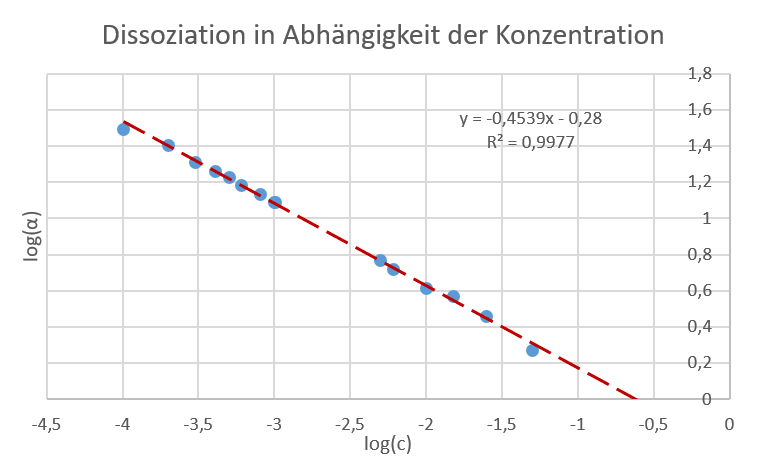
\includegraphics[scale=.7]{../src/img/graph1_25C.png}
    \caption{Bestimmung von $\gamma_\pm$ bei 25$^\circ$C}
\end{figure}

Desweiteren kann man aus der Geradengleichung erkennen, dass je geringer die Konzentration der Lösung ist, desto höher ist gleichzeitig
die prozentuale Aktivität, oder anders ausgedrückte - je geringer die Konzentration, desto mehr Teilchen dissoziieren.
Mit diesem Zusammenhang, kann man auch aus der schwachen Säure HAC bei genügend hoher Verdünnung eine starke machen. \\
Eine starke Säure ist dann stark, wenn sie vollständig dissoziiert, also wenn $\alpha[\%] = 100$ ist. Dies kann mit der Geradengleichung der
Regressionsgerade bestimmt werden.

\begin{align*}
    log(\alpha) &= -0,4539 \, \log(c) - 0,28 \\
    10 &= -0,4539 \, \log(c) - 0,28  \\
    c &= 10^{-23.03} = 2.25 \cdot 10^{-23} \, [mol/kg]
\end{align*}

Bei einer Konzentration von $2.25 \cdot 10^{-23} \, [mol/kg]$ würde Essigsäure bei 25$^\circ$C vollständig dissoziieren.

\subsection{Debye-Radius bei 25$^\circ$C}

Der Debye-Radius gibt an, ab welcher Distanz nur noch $\frac{1}{e}$ der Coulomb-Kraft wirkt und er wird berechnet über:

\begin{align*}
    r_D &= \sqrt{ \frac{\epsilon _0 \epsilon _{rel} k_B T}{2N_A e^2 I}} \\
    k_B &= \frac{R}{N_A} \\
    F &= N_A e
\end{align*}

\begin{align}
    r_D = \sqrt{ \frac{\epsilon _0 \epsilon _{rel} R T}{2 F^2 I}}
\end{align}

Für die Ionenstärke $I = \frac{1}{2} \sum c_i z_i^2$ wir statt c die Aktivität a eingesetzt und da Essigsäure zu gleichen Teilen zerfällt
ist $I = \frac{1}{2} (2 \cdot a) = a$. Unter der Annahme, dass die Konzentration  viel geringer als der Aktivitätskoeffizient ist kann man
($I = a = \gamma _\pm \cdot b = b$) die Ionenstärke in nächster Näherung mit der Molalität b gleichsetzen.

% Table generated by Excel2LaTeX from sheet 'Tabelle1'
\begin{table}[H]
  \centering
  \caption{Debye-Radius von Essigsäure bei 25$^\circ$C}
    \begin{tabular}{lrr}
    \toprule
    \textbf{Lösung} & \multicolumn{1}{l}{\boldmath{}\textbf{Ionenstärke [$mmol/m^3$]}\unboldmath{}} & \multicolumn{1}{l}{\textbf{Debye-Radius [nm] }} \\
    \midrule
    A1    & 50,01 & 43,0 \\
    A2    & 25,01 & 60,8 \\
    A3    & 15,06 & 78,4 \\
    B1    & 10,06 & 95,9 \\
    B2    & 6,05  & 123,7 \\
    A4    & 5,01  & 135,9 \\
    B3    & 1,00  & 303,5 \\
    A5    & 1,00  & 304,6 \\
    C1    & 0,80  & 339,1 \\
    C2    & 0,61  & 390,4 \\
    B4    & 0,51  & 427,9 \\
    C3    & 0,41  & 476,6 \\
    C4    & 0,30  & 554,7 \\
    B5    & 0,20  & 679,2 \\
    C5    & 0,10  & 957,4 \\
    \bottomrule
    \end{tabular}%
  \label{tab:addlabel}%
\end{table}%
 

Um den Zusammenhang zwischen Konzentration und Debye-Radius zu verdeutlichen wurde in Abbildung 2 der logarithmiert rD gegen die logarithmiert Molalität
aufgetragen.

\begin{figure}[H]
    \centering
    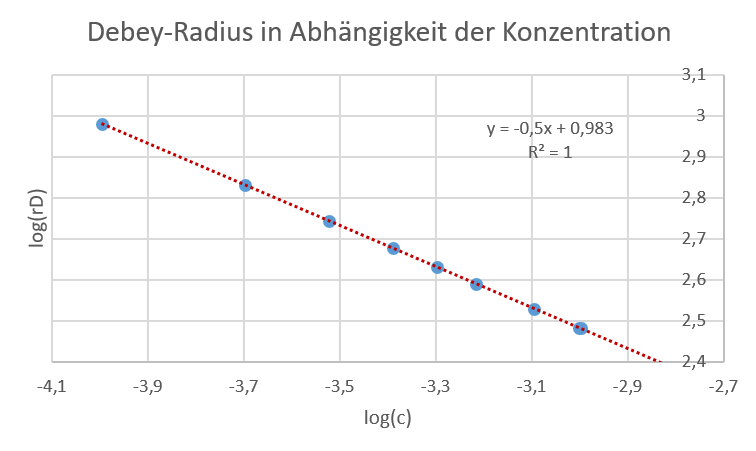
\includegraphics[scale=.7]{../src/img/graph2_25C.png}
    \caption{Debye-Radius bei 25$^\circ$C}
\end{figure}

Wie vorher bei der Dissoziation, erhöht sich auch der Debye-Radius bei geringerer Konzentration. Dies kann man sich durch eine einfache 
Überlegung erklären:
\begin{quote}
    Bei geringerer Konzentration sind die Essigsäuremoleküle nicht so nah beisammen, sie werden also weniger stark abgeschirmt.
\end{quote}

